%!TEX root = ../template.tex
%%%%%%%%%%%%%%%%%%%%%%%%%%%%%%%%%%%%%%%%%%%%%%%%%%%%%%%%%%%%%%%%%%%%
%% chapter3.tex
%% NOVA thesis document file
%%
%% Chapter with a short latex tutorial and examples
%%%%%%%%%%%%%%%%%%%%%%%%%%%%%%%%%%%%%%%%%%%%%%%%%%%%%%%%%%%%%%%%%%%%

\typeout{NT FILE chapter3.tex}%


\chapter{Materials and Methods}
\label{cha:materials_and_methods}


\textit{The following section describes the workflow of the benchmarking study. It begins by describing the input data used, both transcriptomic data and prior knowledge data. Further emphasis is given to the implementation of the selected algorithms. Finally, the description of the algorithm's execution, as well as the methods used to assess their performance.}


\section{Benchmarking architecture setup} % (fold)
\label{sec:benchmarking_architecture_setup}
Several tools and algorithms are available for most research tasks in computational biology, and new algorithms and tools are published every week. Systematic benchmarking of tools is a time- and resource-consuming endeavor, while a lack of benchmarking carries several potential risks. Finding the right computational tool for a given research question is essential. Researchers usually carry out published benchmarking to demonstrate that their tool performs better than others. ABC is a consortium created in 2021 that aims to help members reduce R\&D risks, saving time and resources by distributing the effort of benchmarking computational biology algorithms. ABC is a consortium established in 2021 that aims to assist members in reducing R\&D risks, saving time and resources by distributing the effort of benchmarking computational biology algorithms. ABC maintains the same workflow regardless of the case study. It consists of three main steps: (1) Voting, (2) Curation, and (3) Coding. The consortium members suggest and vote on the use case (1). Once the use case is determined, the curation phase begins, where Clarivate collects the most appropriate datasets and algorithms according to the voted use case (2). Again, the members vote on the final selection of datasets and algorithms (1). Finally, the last phases - implementation, execution, and reporting - are conducted by Clarivate (3). 
The project description will fall within the third phase of the workflow, specifically concerning some of the algorithm's implementation and execution, where I actively participated since all the data was already collected and voted on when I started the project. A visual representation of the study workflow is provided~\ref{fig:fig4} and will be explained in detail in the following sections. The entire workflow was implemented in \gls{R} Statistical Software (v4.4.1) [96].

\begin{figure}[htbp]
    \centering
    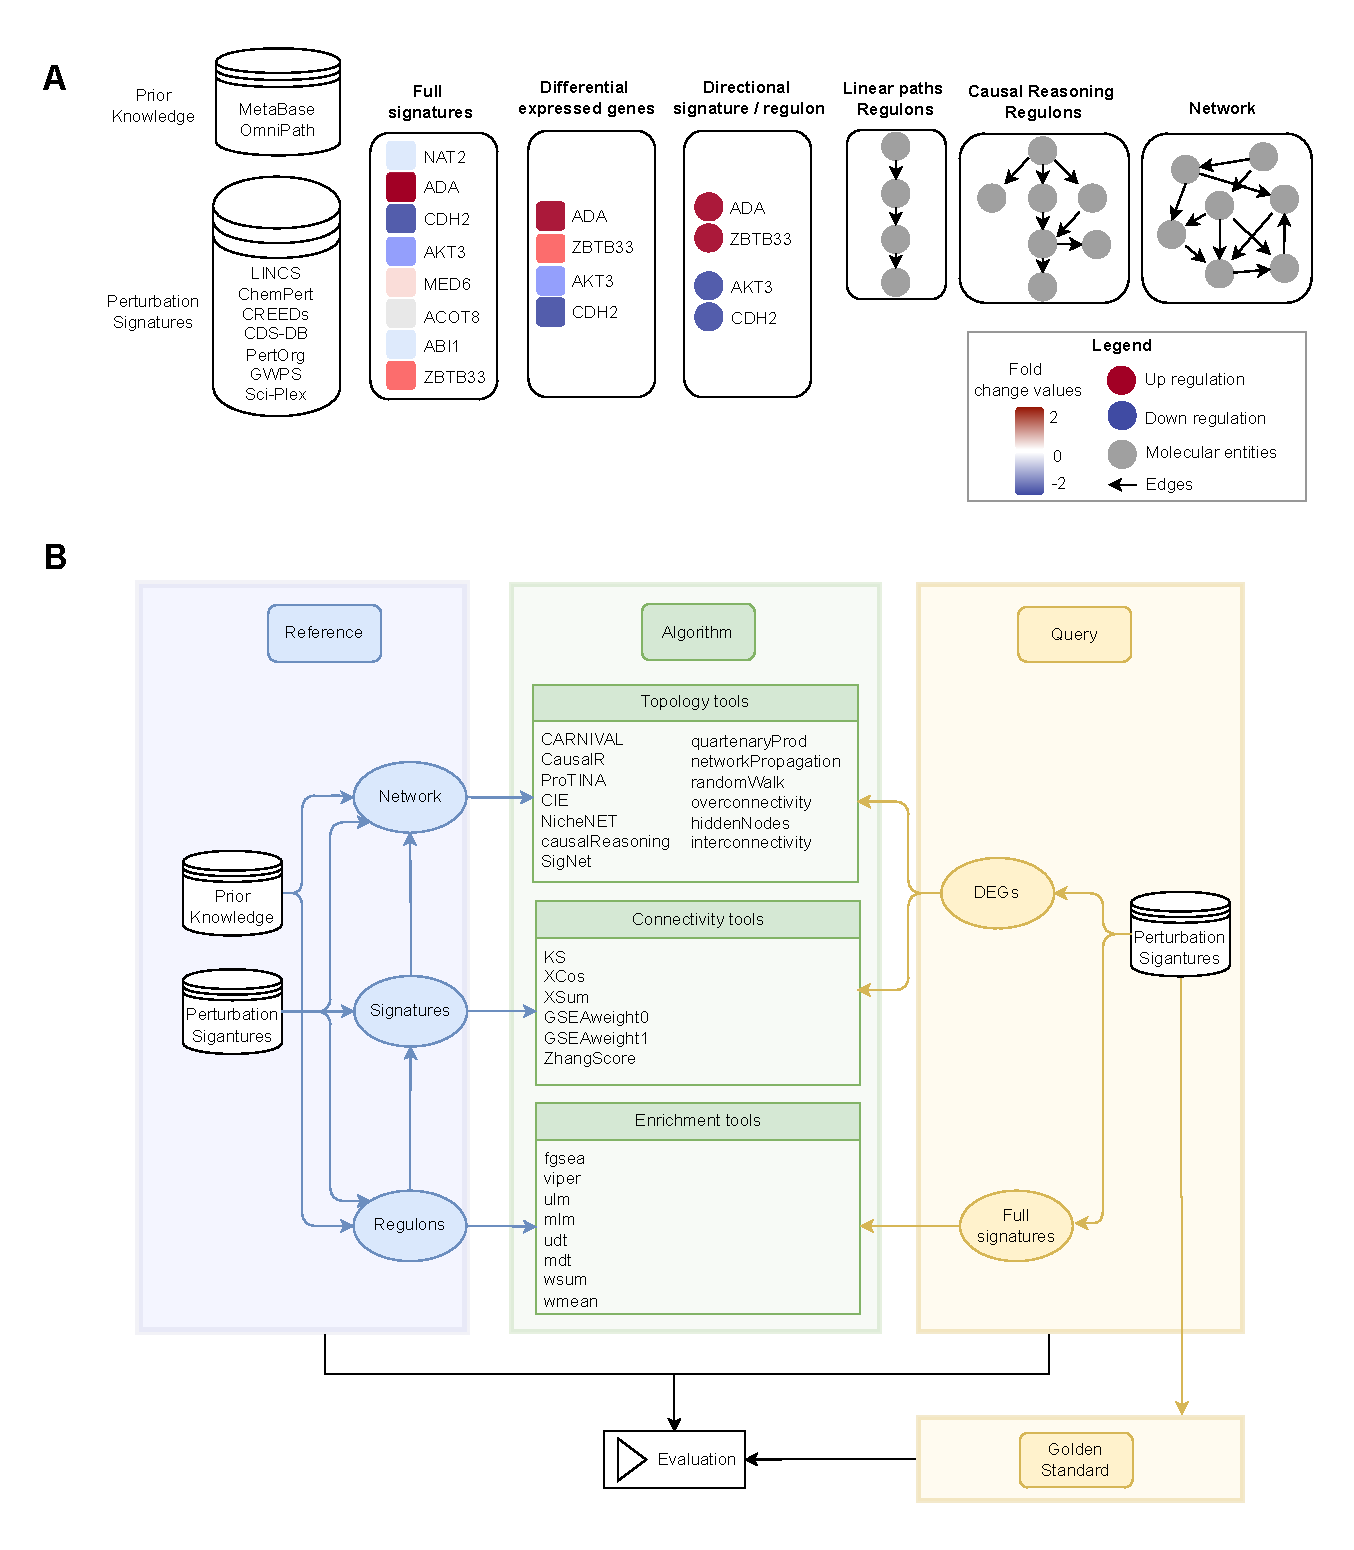
\includegraphics[height=6in]{ABC_workflow}
    \caption{Schematic of the study architecture. A. Perturbation signatures collected from seven public sources are used in the benchmarking framework either as reference, query, and gold standard (known targets) datasets. Prior knowledge networks, used as reference, were derived from two sources: OmniPath (public) and MetaBase™ (commercial). From OmniPath, a global network, and regulons were used as references. From MetaBase, it was also used a full network, regulons, and, in addition to the regular regulons, regulons derived from linear paths. B. Three classes of computational methods were evaluated: topology-based, connectivity-based, and enrichment-based, comprising a total of 27 algorithms. Depending on the method, input data may consist of a global interactome (network), curated signaling pathways, or perturbation signatures (typically directional gene sets or full transcriptomic profiles, which can be reduced to gene sets if needed). These input types are often interrelated, and the arrows in the diagram indicate the required data transformations specific to each algorithm. The output of each method is systematically compared to the gold standard targets for evaluation.}
    \label{fig:fig4}
\end{figure}


\section{Data Description} % (fold)
\label{sec:data_description}

As represented in Figure~\ref{fig:fig4}, each algorithm should receive two types of inputs: query and reference dataset. The query dataset refers to the data derived from perturbed signatures (Full profiles or DEGs lists). The reference dataset can be derived either from perturbed signatures (Full profile, DEGs, or directional/regulons) or from prior knowledge (Networks or pathways/gene sets). The databases and datasets used as perturbed signatures and as prior knowledge are described below.

\subsection{Gene expression data: Perturbation signatures}
\label{sub:gene_expression_data_perturbation_signatures}

Currently, there are several publicly available perturbation-driven gene expression datasets. This study comprehends transcriptomic datasets from 10 different public sources, summarized in Table~\ref{tab:gene_expression_datasets}. Chemical and genetic perturbagens were included, analyzed by bulk microarray, bulk RNA seq, and single-cell RNA seq assays. Each dataset contains more than hundreds of perturbation signatures. For each collection, the perturbagen type, the total number of unique perturbagens profiled, and the subset for which a gold standard target annotation is available were recorded. The gold standard is necessary for the evaluation and it consists of a set of known targets (drug-protein interactions or genes deliberately perturbed), used to assess the ability of the algorithms to recover true upstream regulators from observed expression changes. 
The LINCS expands upon the original CMap by leveraging the cost-effective L1000 platform, which directly measures 978 “landmark” transcripts and imputes the remaining transcriptome to reconstruct genome-wide expression profiles. LINCS comprises several distinct collections of perturbations in human cell lines: over 30,000 unique small-molecule treatments, CRISPR knockouts targeting 5,156 genes, cDNA overexpression of 3,780 genes, and shRNA knockdowns of 4,854 genes. The level 5 data were retrieved from the CLUE platform (available at \href{https://clue.io/data/CMap2020#LINCS2020}{CLUE}). This level already contains the differential expression signatures with z-scores aggregated across biological replicates without p-values. Since each perturbagen usually appears under multiple conditions (different doses, time points, and cell lines), these were condensed into a single consensus signature per perturbagen by extracting every available gene's z-score and then using the median value across signatures. For the gold standard, directional effects were assigned as follows: for chemical perturbations CDDI annotations were used to identify molecular targets inhibited by specific compounds; for CRISPR and shRNA datasets, the target genes were assigned with inhibition effect, and for OE, each target was assigned with activation effect.
ChemPert is a manually curated compendium of 82,256 transcriptional signatures derived from non-cancer cell compound perturbation experiments. Most signatures originate from bulk expression studies in various cell lines, and each is represented as a list of DEGs indicating only up- or down-regulation (no fold-change values or p-values). From the total number of signatures, only 2,587 have distinct compounds. A set of consensus DEG lists were derived to reduce redundancy and runtime. For each compound, only genes appearing as DEGs in at least two signatures and with the same regulation direction were kept. As well as only signatures with at least 50 consensus DEGs. This resulted in 1,304 signatures which was the dataset used instead of the original ChemPert.
CDS-DB contains 78 cancer patient-derived, paired pre- and post-treatment transcriptomic datasets, all with associated metadata such as drug dosages, sampling times, and locations. 181 study-level gene perturbation signatures (85 therapeutic regimens across 39 cancer subtypes) were extracted. The perturbagen consists of drugs, and the expression is measured by microarray or RNA-Seq (including fold change and p-values). 
The sci-Plex dataset is based on a single-cell transcriptomics method that uses nuclear hashing. Sci-Plex dataset profiled three cancer cell lines treated with 188 small-molecule compounds. The data contains full transcriptomic signatures with around 11,000 genes each, containing dose-response effect estimates and associated p-values. Only signatures linked to compounds with known CDDI targets were kept. For each of the 135 perturbagen with a target, the gene expression responses were measured across 3 cell lines, resulting in 405 signatures. 
CREEDS is a crowd-sourced, manually curated collection of perturbation signatures from GEO. Includes both small-molecule and genetic perturbations in mouse and human with the expression from different bulk gene expression platforms. These signatures are represented as DEG lists indicating the regulation direction without fold change values. Only perturbations with CDDI target annotations were retained, and all mouse data were mapped to human orthologs, using the metabaser package.
PertOrg is a curated collection of in vivo genetic perturbation (such as knockdown, knockout, and overexpression) signatures across eight model organisms. Only mouse signatures with more than 5,000 genes were kept and mapped to human orthologs. For the golden standard, perturbation effects were considered as activation in the case  of knock-in, overexpression and activation, and inhibition for all the remaining ones. Since PertOrg originally contained 7,398 signatures but only 2,321 distinct target genes, a filtering criteria was applied. Each signature should have at least 50 DEGs, and the target gene's fold change should be ranked in the top 5% by absolute value among all measured genes within that signature. Then, the selected signature was the one with the highest number of DEGs per target and perturbation type combination. This resulted in 951 signatures used as PertOrg dataset.
The GWPS dataset represents a large-scale effort for single-cell CRISPRi profiling across more than 2.5 million human cells. It targets 9,866 genes and was generated using the 10x Genomics platform. The dataset includes 1,946 perturbation signatures corresponding to gene knockdowns. Each signature consists of full transcriptomic profiles by z-scores without p-values. Although the DEGs per signature were also provided by the authors, only the full signatures were used in the analysis.

% Please add the following required packages to your document preamble:
% \usepackage{longtable}
% Note: It may be necessary to compile the document several times to get a multi-page table to line up properly
\begin{longtable}[c]{lllllll}
\caption{Summary of gene expression datasets used in this study. Each dataset includes transcriptomic signatures derived from chemical or genetic perturbations. The “Perturbagen” column specifies the type of compound or gene perturbation applied, while the “Type” column labels it as either chemical or genetic. The number of perturbagens refers to the unique compounds or genes perturbed in the dataset. The signatures with the golden standard column indicate how many signatures have associated targets that can be used for benchmarking. The signature type describes the format and content of the signature, such as full profiles or DEG lists.}
\label{tab:gene_expression_datasets} \\

\textbf{Data set} &
  \textbf{Perturbagen} &
  \textbf{Type} &
  \textbf{Number of perturbagens} &
  \textbf{Signatures with golden standard} &
  \textbf{Signature type} &
  \textbf{Ref.} \\
\endfirsthead
%
\endhead
%
LINCS compounds & Compound (small molecules)                            & Chemical & 33627 & 3540 & Full              & ~\cite{RN30} \\
ChemPert &
  Compound (small molecules, ligands, drugs) &
  Chemical &
  2508 &
  1304 &
  DEGs (up/down gene sets) &
  ~\cite{RN86} \\
CDS-DB          & Compound (small molecules) Patient-derived            & Chemical & 181   & 181  & Full              & ~\cite{RN84} \\
Sci-Plex        & Compound (Single cell; Different doses)               & Chemical & 189   & 405  & Full (scRNA-seq ) & ~\cite{RN88} \\
CREEDs &
  Disease, small molecules, single gene perturbations &
  Chemical Genetic &
  3051 (875 drugs, 2176 genes) &
  2642 &
  DEGs (up/down gene sets) &
  ~\cite{RN87} \\
LINCS CRISPR    & CRISPR KO                                             & Genetic  & 5156  & 5156 & Full              & ~\cite{RN30} \\
LINCS OE        & cDNA over-expression                                  & Genetic  & 3780  & 3780 & Full              & ~\cite{RN30} \\
LINCS shRNA     & shRNA interference                                    & Genetic  & 4854  & 4854 & Full              & ~\cite{RN30} \\
PertOrg         & shRNA interference; CRISPR knockdown; Over-expression & Genetic  & 7398  & 951  & DEGs              & ~\cite{RN85} \\
GWPS            & CRISPR interference                                   & Genetic  & 1946  & 1946 & Full (scRNA-seq ) & ~\cite{RN89}
\end{longtable}

%\includegraphics[width=0.9\linewidth]{Chapters/Figures/lincs_shrna_a375_head(signature)}\hfill

The concept of causal inference can be described as the ability of algorithms to find the target candidates of a perturbation, in this study, based on gene expression data. Each dataset described in this section feeds into the benchmarking workflow as the query or reference dataset and as a gold standard (signature associated with the set of known targets). Golden standard target annotations are mandatory, not for running the algorithms, but for the evaluation step. During the evaluation, the performance of each algorithm will be assessed based on how well the target was recovered. When using signatures derived from drug perturbation, it can be hard to identify the exact compound used just from gene expression. Instead, it's easier and more meaningful to infer the target(s) of the compound (e.g., a protein the drug binds to). Although MetaBase also contains compound information, most networks do not, but they do include gene or protein targets. Even for connectivity scoring methods, knowing the drug targets helps when querying compound perturbations versus gene perturbation references (or vice versa). Five chemical perturbation datasets (LINCS compounds, ChemPert, CDS-DB, Sci-Plex, and CREEDs) were subjected to this mapping through three approaches. (1) The authors' target information was extracted from the dataset/database whenever possible. All target gene symbols were extracted. (2) Small molecules were mapped against the drugs in Clarivate's CDDI database. (3) The target lists from the database and from CDDI were then merged to form the final set of targets for each drug or small molecule.


\begin{figure}[htbp]
    \centering
    \includegraphics[height=2in]{lincs_shrna_a375_head(signature)}
    \caption{Transctipotomic signatures perturbation from LINCS shRNA, cell line a375.}
    \label{fig:example_signatures}
\end{figure}



\subsection{Prior Knowledge: Interaction Networks} % (fold)
\label{sec:prior_knowledge_interaction_networks}

One type of input that can serve as a reference is prior knowledge data for contextualizing gene expression signatures. 
The benchmarking framework depends on three complementary types of this data: 
PKN (global interaction networks), regulons (regulator-target gene sets), and pathway-derived linear maps (Table~\ref{tab:table4}). 
Although these resources vary in their coverage, they are related, as illustrated in Figure 4. Including sources of different 
sizes and densities is particularly important for understanding how topology-based algorithms manage that in terms of performance. 
Additionally, an increase in network size can introduce noise that may disturb the rationale. 


% \usepackage{graphicx}
\begin{table}[]
\centering
\caption{Summary table of OmniPath and MetaBase prior knowledge resources. Number of nodes and edges are displayed for each resource. Network refers to the full interaction network, while regulons and linear path regulons are downstream-derived, regulators subsets. The regulator and target columns correspond to the number of source and corresponding target nodes, respectively. Gene space counts how many of those nodes correspond specifically to genes (not proteins or others). The three edge-type columns indicate the number of activation, inhibition, or transcriptional regulation interactions. The total number of interactions for each resource is under total column.}
\label{tab:table4}
\resizebox{\textwidth}{!}{%
\begin{tabular}{lllllllll}
\multicolumn{2}{l}{}                             & \multicolumn{3}{l}{Nodes}       & \multicolumn{4}{l}{Edges}                                         \\
\multicolumn{2}{l}{Resource}                     & Regulator & Target & Gene space & Activation & Inhibition & Transcriptional regulation & Total      \\
\multirow{2}{*}{OmniPath} & Network              & 6,166     & 6,723  & 7,809      & 119,113    & 13,680     & 64,367                     & 145,896    \\
                          & Regulons             & 4,442     & 6,723  & 5,622      & 5,842,390  & 4,270,032  & 10,112,422                 & 10,112,422 \\
\multirow{3}{*}{MetaBase} & Network              & 3,3927    & 1,5229 & 1,7693     & 81,866     & 61,214     & 101,752                    & 657,746    \\
                          & Regulons             & 1,1739    & 1,0476 & 9,988      & 23,844,526 & 21,469,352 & 45,313,878                 & 45,313,878 \\
                          & Linear Path Regulons & 2,922     & 9,465  & 3,185      & 3,493,007  & 1,361,149  & 4,854,156                  & 4,854,156 
\end{tabular}%
}
\end{table}



\section{Algortithms} % (fold)
\label{sec:algorithms}

To carry out a systematic and robust comparative evaluation of inference algorithms, wrapper functions were developed to standardize the input data 
and output formatting in different computational approaches. Each algorithm has specific data requirements and processing methods, requiring 
adaptation to ensure compatibility in the common framework. A wrapper is nothing more than a function that serves as an intermediary layer. 
These are important to handle data type conversions, parameter standardization, and result formatting, allowing diverse algorithms to be executed 
consistently regardless of their underlying implementation differences. This approach addresses the inherent complexity of having algorithms coming 
from different approaches. Here there are two types of wrappers: shared and individual. The shared wrapper architecture incorporates an already 
established package that bundles several algorithms inside, unlike the individual ones that incorporate single algorithms. The connectivity mapping 
approaches from the RCSM package, enrichment methods from decoupleR, and topology-based algorithms from CBDD were implemented in shared wrappers. 
On the other hand, causal reasoning CARNIVAL, CausalR, ProTINA, CIE, and NicheNet were incorporated in individual wrappers. Table 5 provides a 
complete list of algorithms together with their annotations.
Some supporting helper functions were also implemented to facilitate essential data conversions across all wrappers. Those functions include mapping 
identifiers between transcriptomic datasets and network nodes to ensure the same IDs and converting the input data when necessary. For the query 
input data, the tool may need a full signature or DEGs. When DEGs are required, the full signature can be filtered using a fold change and p-value 
threshold or by simply taking the top threshold for differentially expressed genes by fold change magnitude. Regarding reference, the workflow can 
start with PKN or full signatures, and for topology, enrichment, and CMap tools, require networks, regulons/gene sets, and full signatures, respectively. 
To use this large variety of input data and tools, some conversions are required to run them uniformly. All the conversions are indicated by the 
arrows in Figure 4 B. The parameters selected for each algorithm can be found in Supplementary table 2. 
As the input data, the output should also have the same format, so it is possible to evaluate the performance of each algorithm. For that reason, 
at the end of each run, all algorithm wrappers return a table with all prioritized regulators identified without any significance filtering applied. 
The output contains a score column, and the larger score reflects greater confidence in this regulator being causal for observed differential 
expression patterns. Score may be signed if the tools can predict directionality of perturbation. In that case, regulators are ranked by absolute 
value of score, and activation/repression status is stored in separate column effect (-1/1 values). 



The Table~\ref{tab:algorithm_summary} provides a summary of the algorithms used in the study.

%% If I need to change this table to a horizontal layout, just uncomment the next line and the line after the table:
%% \begin{newpdflayout}{210mm}{297mm}%{420mm}

\bgroup
%\rowcolors{1}{}{GhostWhite}
\begin{xltabular}{\textwidth}{Xcccccc}
\caption{Algorithm summary.}
\label{tab:algorithm_summary}\\
\toprule
%\rowcolor{Gainsboro}%
\textbf{Tool}  & \textbf{Algorithm}   & \textbf{Description}   & \textbf{Resource}   & \textbf{Dataset}   & \textbf{Reference}   \\
\midrule
\multicolumn{6}{l}{\textbf{Causal Reasoning}} \\
CARNIVAL            & Description  & Network    & DEG/Full  & ~\cite{RN41} \\
CausalR             & Description  &            &           & ~\cite{RN32} \\
ProTINA             & Description  &            &           & ~\cite{RN80} \\
CIE                 & Description  &            &           & ~\cite{RN81} \\
NicheNet            & Description  &            &           & ~\cite{RN42} \\
causalReasoning     & Description  &            &           & ~\cite{RN36} \\
Signatures          & Description  &            &           & ~\cite{RN36} \\
quaternaryProd      & Description  &            &           & ~\cite{RN36} \\    
\midrule
\textbf{Causal Reasoning (baseline)} \\
randomWalk          & Description  & Network    & DEG/Full  & ~\cite{RN36} \\
networkPropagation  & Description  &            &           & ~\cite{RN36} \\
overconnectivity    & Description  &            &           & ~\cite{RN36} \\
hiddenNodes         & Description  &            &           & ~\cite{RN36} \\
interconnectivity   & Description  &            &           & ~\cite{RN36} \\
overconnectivity    & Description  &            &           & ~\cite{RN36} \\
\midrule
\textbf{CMap} \\
KS             & Description & Signatures   & DEG/Full     & ~\cite{RN79} \\
XCos           & Description &              &              & ~\cite{RN79} \\
XSum           & Description &              &              & ~\cite{RN79} \\
ZhangScore     & Description &              &              & ~\cite{RN79} \\
GSEAweight0    & Description &              &              & ~\cite{RN79} \\
GSEAweight1    & Description &              &              & ~\cite{RN79} \\
\midrule
\textbf{Enrichment} \\
wmean   & Description  & Regulons     & Signatures  & ~\cite{RN36} \\
fgsea   & Description  &              &             & ~\cite{RN35} \\
viper   & Description  &              &             & ~\cite{RN35} \\
ulm     & Description  &              &             & ~\cite{RN36} \\
mlm     & Description  &              &             & ~\cite{RN36} \\
udt     & Description  &              &             & ~\cite{RN36} \\
mdt     & Description  &              &             & ~\cite{RN36} \\
wsum    & Description  &              &             & ~\cite{RN35} \\
%\rowcolor{Gainsboro}%
\bottomrule
\end{xltabular}
\egroup



\subsection{Connectivity Mapping} % (fold)
\label{sub:connectivity_mapping}

The~\ref{fig:fig5} represents the wrapper function framework for running connectivity mapping algorithms from the RCSM package [87]. This package provides uniform implementations of several CMap scoring methods including Kolmogorov-Smirnov (KS), and GSEA-based approaches. The function is designed to accept filtered DEG lists as query input and full perturbation signatures as reference data. If full signatures are used as the query, they are converted to DEGs using the filtering parameters (Supplementary table 2), as well as the additional parameters. RCSM R package includes a variety of algorithms already implemented, each designed to quantify the similarity or dissimilarity between query and reference perturbation signatures. Those algorithms include the Kolmogorov-Smirnov (KS) statistic which was used in the original Connectivity Map [9]; Xcos, a cosine similarity metric between query and reference fold-changes; Xsum connectivity map statistic based on the sum of reference fold-change values of query genes; GSEAweight0 is a GSEA weighted KS  ES with parameter p = 0, meaning that the fold-change magnitude is not taken into account; GSEAweight1 with parameter p = 1, fold-change magnitude contributes linearly; Zhang, a connectivity mapping score first suggested in [105].
The function handles the different algorithm requirements by preparing either separate up- and down-regulated gene lists for most methods or simple gene vectors for XCos. The function also includes optional regulator filtering for TF mode. The output is formatted to return regulator rankings with similarity scores, directional effects, and optional statistical significance measures. The results are sorted by absolute score magnitude to prioritize the most relevant regulatory relationships regardless of similarity direction. For these algorithms, the regulator score measures the similarity of the query versus the reference perturbation signature.

\begin{figure}[htbp]
    \centering
    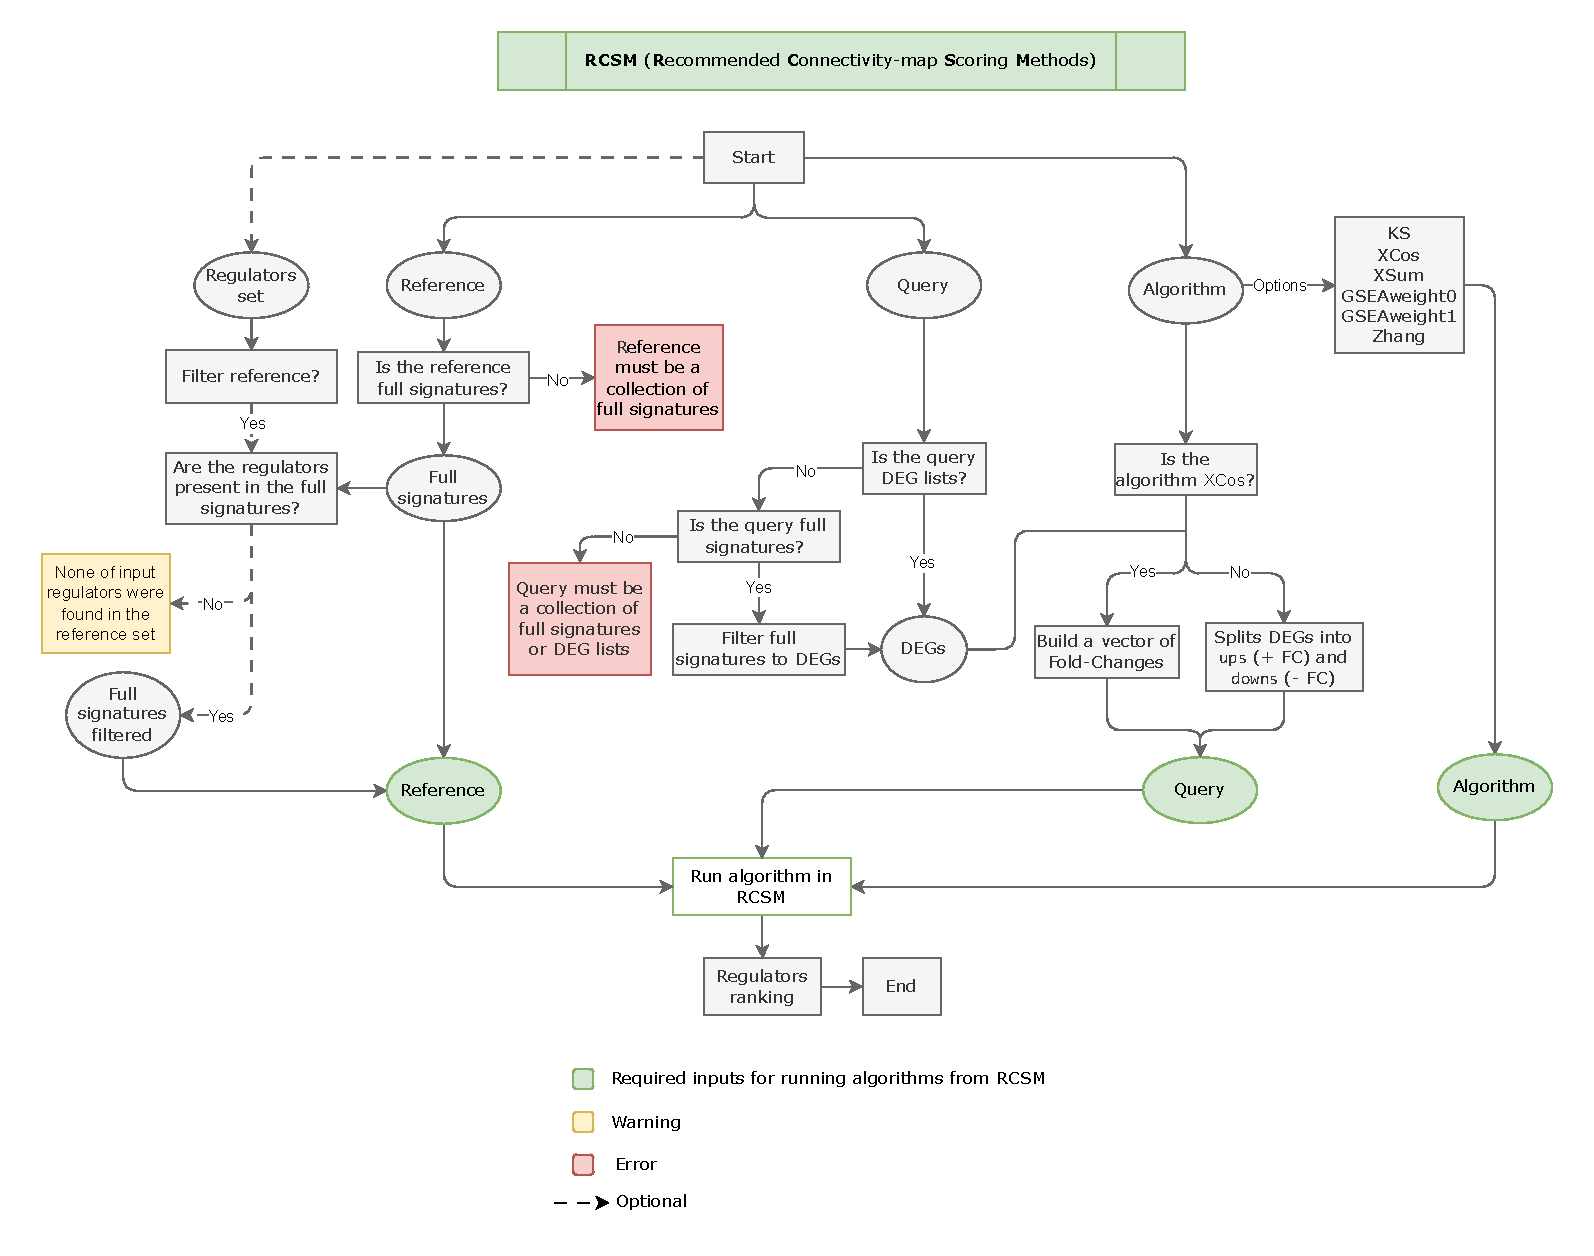
\includegraphics[height=5in]{RCSM}
    \caption{Flowchart representing the main steps for implementing connectivity mapping algorithms pre-built in the RCSM R package. The general computational pipeline for executing connectivity-based methods, showing the main input requirements, data preprocessing steps, algorithm execution, and output generation. Green indicate required inputs, while red highlight potential errors.}
    \label{fig:fig5}
\end{figure}
%\end{newpdflayout}



\subsection{Pathway Enrichment} % (fold)
\label{sub:pathway_enrichment}


For running the enrichment-based algorithms, the decoupleR package [10] was used. 
It contains 12 algorithms already implemented to extract biological activities from omics data using prior knowledge resources (gene sets or regulons).
Some of them take directionality into account (i.e., can work with regulon-gene set with activated and repressed genes). 
The package was initially used to benchmark approaches for TF activity inference. From those, only GSEA and the others that respect directionality 
were used. As for connectivity-mapping algorithms, a shared wrapper function (Figure~\ref{fig:fig6}) was built to prepare the input and 
output data for these algorithms. It is designed to accept full signatures as query and regulon table or a gene regulatory network as reference data. 
If the reference is a list of signatures or DEGs, it is converted to directed regulatory networks using the common filtering parameters described above. 
The implementation supports TF-mode by filtering the network to keep only transcription-regulation edges. The query signatures are converted to an 
fold change matrix and perform ID space conversions when necessary to match network node identifiers. 

\begin{figure}[htbp]
    \centering
    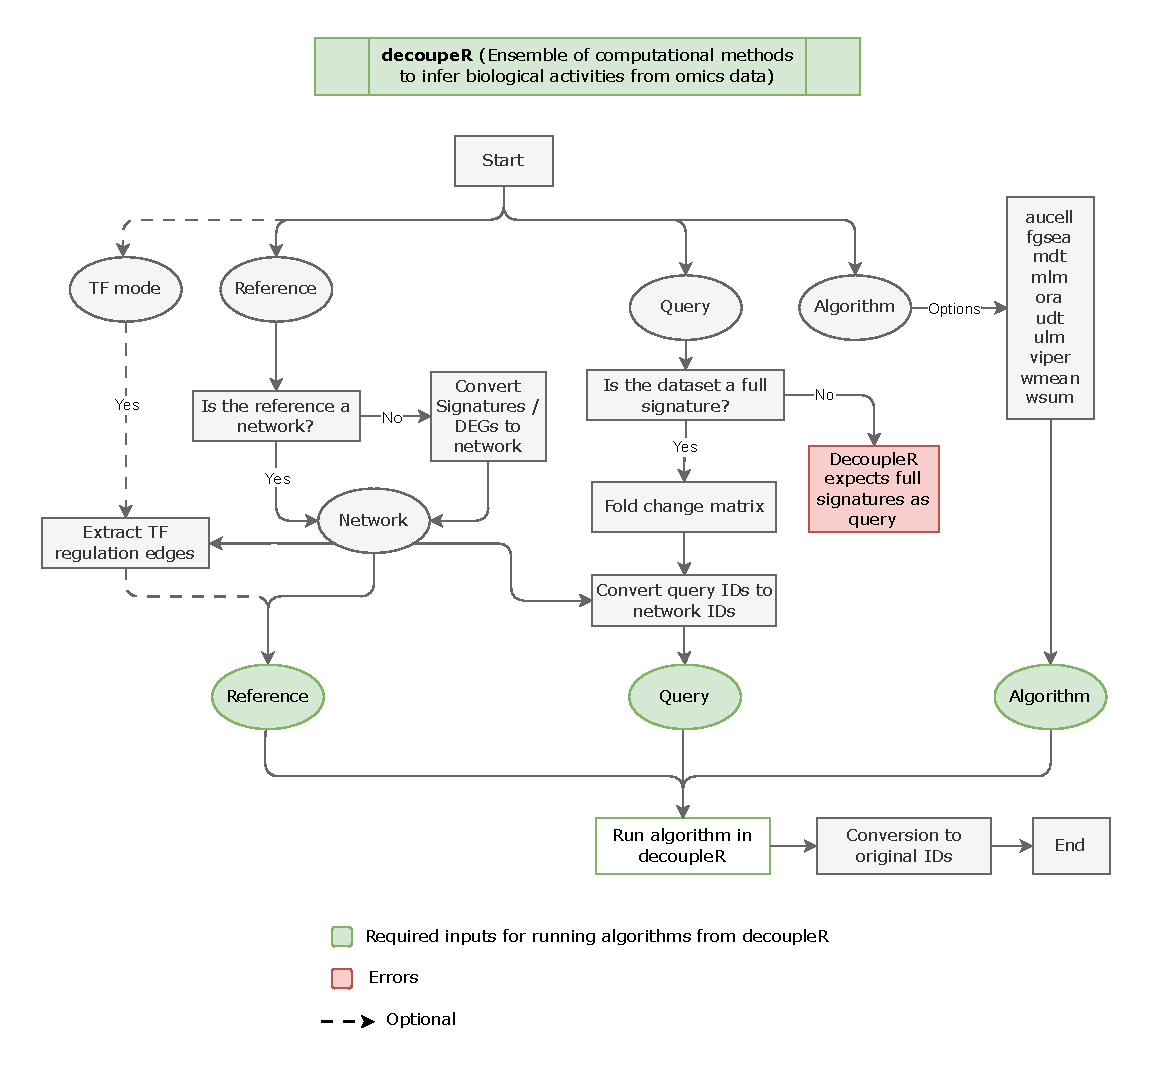
\includegraphics[height=5in]{decoupleR}
    \caption{Flowchart representing the main steps for implementing enrichment algorithms pre-built in the decoupleR package. The general computational pipeline for executing enrichment-based methods, showing the main input requirements, data preprocessing. Green indicates required inputs, while red highlights potential errors.}
    \label{fig:fig6}
\end{figure}
%\end{newpdflayout}
